% !TEX TS-program = pdflatexmk
% Lecture 28 -- typeset from the handwritten "28.Apr-1.pdf".
\documentclass[11pt]{article}
\usepackage[letterpaper,margin=1in]{geometry}
\usepackage{amsmath}
\usepackage{amssymb}
\usepackage{xcolor}
\usepackage{tikz}
\usetikzlibrary{decorations.pathmorphing,arrows.meta,patterns,positioning,calc}
\usepackage{enumitem}
\usepackage[hidelinks]{hyperref}
\usepackage{xurl}  % lets the long demo URL break across lines
\setlength{\parindent}{0pt}
\setlength{\parskip}{6pt}

\definecolor{notered}{RGB}{220,40,40}
\definecolor{noteblue}{RGB}{20,110,230}
\newcommand{\topic}[1]{\textcolor{noteblue}{#1}}
% blue circled source label, as in the notes
\newcommand{\circled}[1]{\tikz[baseline=(c.base)]\node[draw=noteblue,thick,circle,inner sep=1.2pt,text=noteblue](c){#1};}

% Lens outlines, height 1.3, centred at the origin of the current scope.
\newcommand{\lensDX}[1][]{\draw[thick,#1] (0,0.65) to[bend left=35] (0,-0.65) to[bend left=35] (0,0.65);}
\newcommand{\lensPX}[1][]{\draw[thick,#1] (0,0.65) -- (0,-0.65) to[bend right=55] (0,0.65);}
\newcommand{\lensMa}[1][]{\draw[thick,#1] (-0.2,0.65) to[bend left=30] (-0.2,-0.65) -- (0.05,-0.65) to[bend right=45] (0.05,0.65) -- cycle;}
\newcommand{\lensMb}[1][]{\draw[thick,#1] (0.2,0.65) to[bend right=30] (0.2,-0.65) -- (-0.05,-0.65) to[bend left=45] (-0.05,0.65) -- cycle;}
\newcommand{\lensPV}[1][]{\draw[thick,#1] (-0.25,0.65) -- (-0.25,-0.65) -- (0.2,-0.65) to[bend left=40] (0.2,0.65) -- cycle;}
\newcommand{\lensDV}[1][]{\draw[thick,#1] (-0.3,0.65) to[bend left=35] (-0.3,-0.65) -- (0.3,-0.65) to[bend left=35] (0.3,0.65) -- cycle;}

\begin{document}

{\Large \underline{Lecture 28}}

\begin{itemize}[label=--]
  \item HW-9 due coming Friday 11\,pm
  \item HW 7--10 will be on Midterm-III
  \item UT Sage
  \item Midterm-III make-up time poll
  \item Midterm-III practice problems
\end{itemize}
\begin{itemize}
  \item DGCX47
\end{itemize}

\bigskip
Goals:
\begin{enumerate}[label=\arabic*.]
  \item Lens maker's formula
  \item Interference of waves
\end{enumerate}

\newpage
% ------------------------------------------------------------------ page 2
\[
  \text{Power} = \frac{1}{f}
  \qquad\qquad
  \begin{array}{l}
    (f \text{ is in m})\\[4pt]
    \left(\begin{array}{l}\text{Power is in}\\ \text{diopters}\end{array}\right)
  \end{array}
\]

Q) \ Power $> -0.25$\,D % CORRECTED: notes had "Q>"

\hspace*{2em}What is the min far point of the eye?

\begin{center}
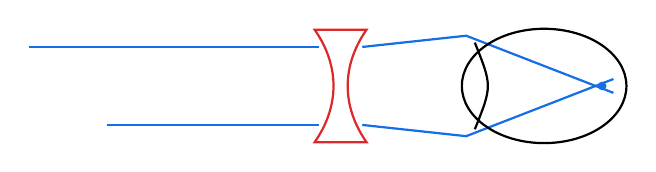
\begin{tikzpicture}[scale=1.1]
  % parallel rays, diverging lens, eye
  \draw[noteblue, thick] (0,0.45) -- (3.35,0.45);
  \draw[noteblue, thick] (0.9,-0.45) -- (3.35,-0.45);
  \begin{scope}[shift={(3.6,0)}] \lensDV[notered] \end{scope}
  \draw[noteblue, thick] (3.85,0.45) -- (5.05,0.58) -- (6.75,-0.08);
  \draw[noteblue, thick] (3.85,-0.45) -- (5.05,-0.58) -- (6.75,0.08);
  \draw[thick] (5.95,0) ellipse (0.95 and 0.66);
  \draw[thick] (5.15,0.5) .. controls (5.35,0) .. (5.15,-0.5);
  \fill[noteblue] (6.62,0) circle (0.05);
\end{tikzpicture}
\end{center}

\[
  d_o = \infty \qquad\qquad\qquad d_i = -d_{\text{far}}
\]
\[
  \frac1f = \frac{1}{d_o} + \frac{1}{d_i}
\]

% ------------------------------------------------------------------ page 3
\begin{align*}
  \frac1f &= \frac1\infty - \frac{1}{d_{\text{far}}}\\[4pt]
  f &= -d_{\text{far}}\\[4pt]
  P = \frac1f &= -\frac{1}{d_{\text{far}}}\\[4pt]
  -\frac{1}{d_{\text{far}}} &> -0.25\\[4pt]
  \frac{1}{d_{\text{far}}} &< 0.25\\[4pt]
  4\,\text{m} &< d_{\text{far}}
\end{align*}

\begin{center}
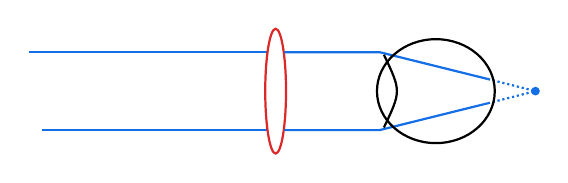
\begin{tikzpicture}[scale=1.1]
  % parallel rays, (converging) lens, eye; rays meet behind the eye
  \draw[noteblue, thick] (0,0.45) -- (2.75,0.45);
  \draw[noteblue, thick] (0.15,-0.45) -- (2.75,-0.45);
  \draw[notered, thick] (2.85,0) ellipse (0.12 and 0.72);
  \draw[noteblue, thick] (2.95,0.45) -- (4.05,0.45) -- (5.3,0.14);
  \draw[noteblue, thick] (2.95,-0.45) -- (4.05,-0.45) -- (5.3,-0.14);
  \draw[noteblue, thick, densely dotted] (5.3,0.14) -- (5.85,0) (5.3,-0.14) -- (5.85,0);
  \fill[noteblue] (5.85,0) circle (0.05);
  \draw[thick] (4.7,0) ellipse (0.68 and 0.6);
  \draw[thick] (4.1,0.42) .. controls (4.3,0) .. (4.1,-0.42);
\end{tikzpicture}
\end{center}

\newpage
% ------------------------------------------------------------------ page 4
{\large \underline{Lens maker's formula}}

\begin{itemize}[label=--]
  \item General formula for determining focal length of non-thin lenses
  % CORRECTED: notes had "determing"
  % CHECK: this is the thin-lens form of the lensmaker's equation; "non-thin" may be meant as
  % "thin" (or "lenses with curved surfaces"). Left as in the notes.
\end{itemize}

\begin{center}
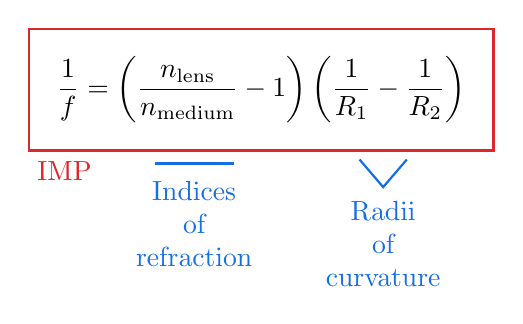
\begin{tikzpicture}
  \node[draw=notered, thick, inner sep=10pt] (F)
    {$\displaystyle \frac1f = \left(\frac{n_{\text{lens}}}{n_{\text{medium}}} - 1\right)\left(\frac{1}{R_1} - \frac{1}{R_2}\right)$};
  \node[notered, anchor=north west] at (F.south west) {IMP};
  \draw[noteblue, thick] ($(F.south)+(-1.35,-0.15)$) -- ($(F.south)+(-0.35,-0.15)$);
  \node[noteblue, align=center, anchor=north] at ($(F.south)+(-0.85,-0.25)$) {Indices\\of\\refraction};
  \draw[noteblue, thick] ($(F.south)+(1.25,-0.1)$) -- ($(F.south)+(1.55,-0.45)$) -- ($(F.south)+(1.85,-0.1)$);
  \node[noteblue, align=center, anchor=north] at ($(F.south)+(1.55,-0.5)$) {Radii\\of\\curvature};
\end{tikzpicture}
\end{center}

\[
  P = \frac1f
\]

\begin{center}
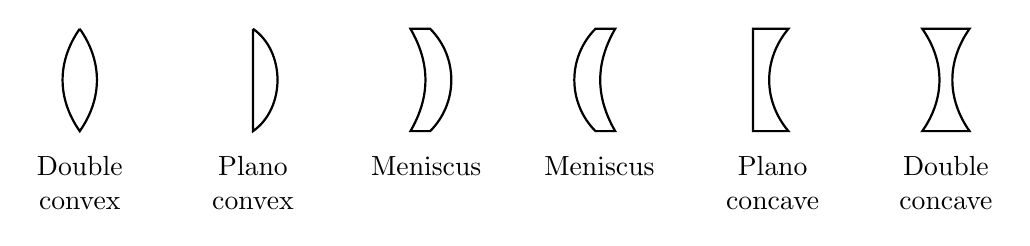
\begin{tikzpicture}
  \foreach \x/\name/\cmd in {0/{Double\\convex}/\lensDX, 2.2/{Plano\\convex}/\lensPX,
                             4.4/{Meniscus}/\lensMa, 6.6/{Meniscus}/\lensMb,
                             8.8/{Plano\\concave}/\lensPV, 11/{Double\\concave}/\lensDV} {
    \begin{scope}[shift={(\x,0)}] \cmd \end{scope}
    \node[align=center, anchor=north] at (\x,-0.85) {\name};
  }
\end{tikzpicture}
\end{center}

\newpage
% ------------------------------------------------------------------ page 5
\begin{center}
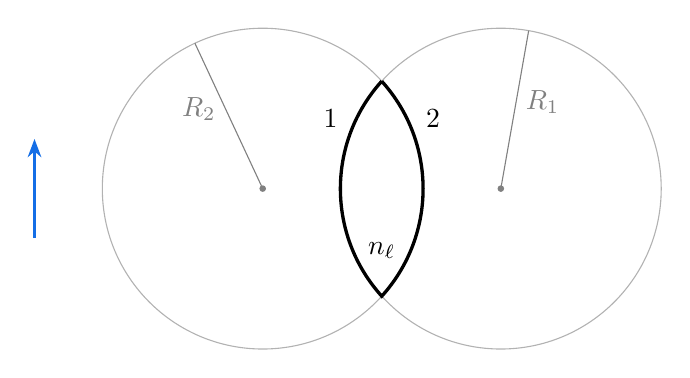
\begin{tikzpicture}[scale=1.05]
  % the two spheres whose surfaces form the lens
  \draw[gray!60] (1.44,0) circle (1.94);
  \draw[gray!60] (-1.44,0) circle (1.94);
  \fill[gray] (1.44,0) circle (0.04);
  \fill[gray] (-1.44,0) circle (0.04);
  \draw[gray] (1.44,0) -- ($(1.44,0)+(80:1.94)$) node[pos=0.55, right] {$R_1$};
  \draw[gray] (-1.44,0) -- ($(-1.44,0)+(115:1.94)$) node[pos=0.55, left] {$R_2$};
  % the lens: surface 1 (left) is part of the right sphere, surface 2 of the left one
  \fill[white] (0,1.3) arc[start angle=137.9, end angle=222.1, radius=1.94]
                       arc[start angle=-42.07, end angle=42.07, radius=1.94];
  \draw[very thick] (0,1.3) arc[start angle=137.9, end angle=222.1, radius=1.94]
                            arc[start angle=-42.07, end angle=42.07, radius=1.94];
  \node at (-0.62,0.85) {1};
  \node at (0.62,0.85) {2};
  \node at (0,-0.75) {$n_\ell$};
  % object
  \draw[noteblue, thick, -{Stealth}] (-4.2,-0.6) -- (-4.2,0.6);
\end{tikzpicture}
\end{center}

\begin{tabular}{@{}l@{\ }l}
  Center of sphere is on left: & $R < 0$\\
  \hspace*{6em}\texttt{"}\hspace*{4.5em} right: & $R > 0$
\end{tabular}

\hspace*{3em}Above example: \ $R_1 > 0$\\
\hspace*{11.3em}$R_2 < 0$

\begin{tabular}{@{}l@{\quad}l}
  $f > 0$ & : Converging lens\\
  $f < 0$ & : Diverging lens
\end{tabular}

\newpage
% ------------------------------------------------------------------ page 6
{\large Alternate heuristic}

\begin{itemize}[label=--]
  \item If side towards object is convex $\Rightarrow R > 0$
\end{itemize}

\hspace*{2em}$\left(\begin{array}{l}
  \text{front of spoon} = \text{convex}\\
  \text{back of spoon} = \text{concave}
\end{array}\right)$

\begin{center}
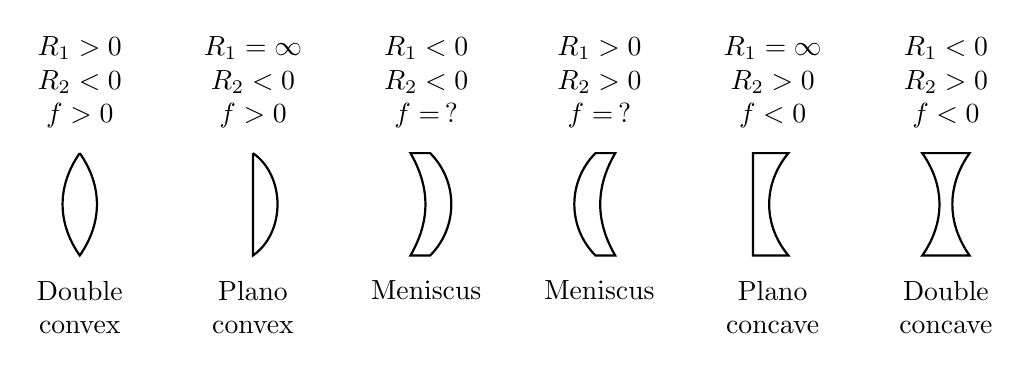
\begin{tikzpicture}
  \foreach \x/\a/\b/\c/\name/\cmd in {
      0/{R_1>0}/{R_2<0}/{f>0}/{Double\\convex}/\lensDX,
      2.2/{R_1=\infty}/{R_2<0}/{f>0}/{Plano\\convex}/\lensPX,
      4.4/{R_1<0}/{R_2<0}/{f=\,?}/{Meniscus}/\lensMa,
      6.6/{R_1>0}/{R_2>0}/{f=\,?}/{Meniscus}/\lensMb,
      8.8/{R_1=\infty}/{R_2>0}/{f<0}/{Plano\\concave}/\lensPV,
      11/{R_1<0}/{R_2>0}/{f<0}/{Double\\concave}/\lensDV} {
    \node[align=center, anchor=south] at (\x,0.85) {$\a$\\$\b$\\$\c$};
    \begin{scope}[shift={(\x,0)}] \cmd \end{scope}
    \node[align=center, anchor=north] at (\x,-0.85) {\name};
  }
\end{tikzpicture}
\end{center}

\begin{itemize}[label=--]
  \item Lenses thinner in the middle are diverging
  \item Lenses thicker in the middle are converging
\end{itemize}

\newpage
% ------------------------------------------------------------------ page 7 (printed problem + handwriting)
{\sffamily
26.8 Lensmaker

The two surfaces of a lens have radii of $r_1 = -20$ \emph{cm} and
$r_2 = +\,5$ \emph{cm}. % the "5" is handwritten over the printed value, which is blacked out
The index of refraction of the lens is $n = 1.52$. What kind lens is it?

\begin{enumerate}[label=\Alph*)]
  \item Converging
  \item Diverging \ \checkmark
  \item Not enough information
\end{enumerate}
}

\[
  \frac1f = \left(\frac{n_{\text{glass}}}{n_{\text{air}}} - 1\right)\left(-\frac{1}{20} - \frac15\right)
  = 0.52\left(-\frac{5}{20}\right)
  \qquad \underline{\underline{f < 0}}
\]

\begin{center}
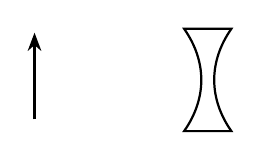
\begin{tikzpicture}
  \draw[thick, -{Stealth}] (0,-0.5) -- (0,0.6);
  \begin{scope}[shift={(2.2,0)}] \lensDV \end{scope}
\end{tikzpicture}
\end{center}

\newpage
% ------------------------------------------------------------------ page 8
{\large \underline{Interference of waves}}

\begin{itemize}[label=--]
  \item Waves are a disturbance in a medium that transmit information/energy through that medium
\end{itemize}

\begin{center}
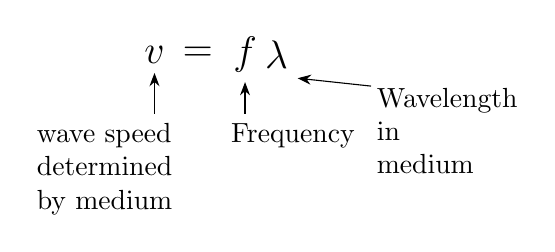
\begin{tikzpicture}
  \node (v) at (0,0) {\Large $v$};
  \node at (0.55,0) {\Large $=$};
  \node (f) at (1.15,0) {\Large $f$};
  \node (l) at (1.55,0) {\Large $\lambda$};
  \draw[-{Stealth}] (0,-0.75) -- (v.south);
  \node[align=left, anchor=north east] at (0.35,-0.75) {wave speed\\determined\\by medium};
  \draw[-{Stealth}] (1.15,-0.75) -- (f.south);
  \node[anchor=north west] at (0.85,-0.75) {Frequency};
  \draw[-{Stealth}] (2.75,-0.4) -- (l.south east);
  \node[align=left, anchor=north west] at (2.7,-0.3) {Wavelength\\in\\medium};
\end{tikzpicture}
\end{center}

\begin{tabular}{@{}l@{\ }l}
  \underline{Constructive}: & Waves overlap in phase,\\ & amplitudes add\\[8pt]
  \underline{Destructive}: & Waves overlap out of phase,\\ & amplitudes subtract
\end{tabular}

\newpage
% ------------------------------------------------------------------ page 9
\begin{itemize}[label=--]
  \item Sources \circled{A} \& \circled{B} emit waves in phase
\end{itemize}

% two in-phase sources; A starts Delta d further along than B; observer on the right
\newcommand{\observer}[1]{%
  \draw[thick] (#1,1.12) circle (0.14);
  \draw[thick] (#1,0.98) -- (#1,0.2) (#1,0.2) -- ++(-0.2,-0.35) (#1,0.2) -- ++(0.2,-0.35)
               (#1-0.2,0.7) -- (#1,0.78) -- (#1+0.2,0.7);}

\begin{center}
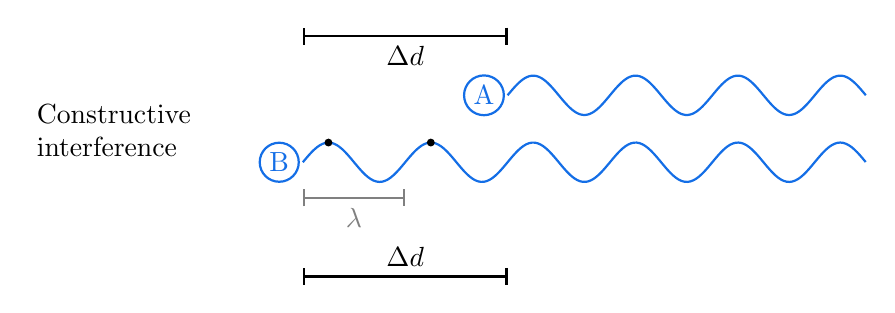
\begin{tikzpicture}
  \node[align=left] at (-1.4,0.4) {Constructive\\interference};
  % wavelength 1.3; A starts Delta d = 2 lambda after B, so they arrive in phase
  \draw[noteblue, thick, domain=1:8.15, samples=200, smooth] plot (\x, {0.25*sin(360*(\x-1)/1.3)});
  \draw[noteblue, thick, domain=3.6:8.15, samples=150, smooth] plot (\x, {0.85+0.25*sin(360*(\x-3.6)/1.3)});
  \node[draw=noteblue, thick, circle, inner sep=1.5pt, text=noteblue] at (0.7,0) {B};
  \node[draw=noteblue, thick, circle, inner sep=1.5pt, text=noteblue] at (3.3,0.85) {A};
  \fill (1.325,0.25) circle (0.05); \fill (2.625,0.25) circle (0.05);
  \observer{7.4}
  \draw[|-|, thick] (1,1.6) -- node[below] {$\Delta d$} (3.6,1.6);
  \draw[|-|, thick, gray] (1,-0.45) -- node[below] {$\lambda$} (2.3,-0.45);
  \draw[|-|, thick] (1,-1.45) -- node[above] {$\Delta d$} (3.6,-1.45);
\end{tikzpicture}

\bigskip
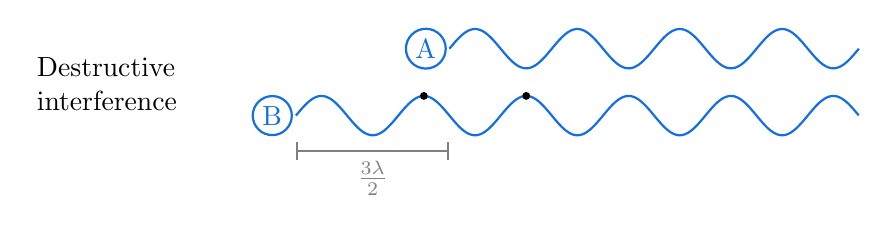
\begin{tikzpicture}
  \node[align=left] at (-1.4,0.4) {Destructive\\interference};
  % A starts 3 lambda / 2 after B, so they arrive out of phase
  \draw[noteblue, thick, domain=1:8.15, samples=200, smooth] plot (\x, {0.25*sin(360*(\x-1)/1.3)});
  \draw[noteblue, thick, domain=2.95:8.15, samples=150, smooth] plot (\x, {0.85+0.25*sin(360*(\x-2.95)/1.3)});
  \node[draw=noteblue, thick, circle, inner sep=1.5pt, text=noteblue] at (0.7,0) {B};
  \node[draw=noteblue, thick, circle, inner sep=1.5pt, text=noteblue] at (2.65,0.85) {A};
  \fill (2.625,0.25) circle (0.05); \fill (3.925,0.25) circle (0.05);
  \draw[|-|, thick, gray] (1,-0.45) -- node[below] {$\frac{3\lambda}{2}$} (2.95,-0.45);
\end{tikzpicture}
\end{center}

\[
  \Delta d = \begin{cases}
    m\lambda & \text{Cons.}\\[6pt]
    \left(m + \tfrac12\right)\lambda & \text{Dest.}
  \end{cases}
\]

Demo link: \url{https://phet.colorado.edu/sims/html/wave-on-a-string/latest/wave-on-a-string_all.html}

\end{document}
